\documentclass[type=dr, dr=rernat, accentcolor=tud7b,colorbacktitle, bigchapter, openright, twoside, 12pt ]{tudthesis}
%\documentclass[11pt,twoside,a4paper]{article}
\usepackage[english]{babel} 
\usepackage[utf8]{inputenc}
\usepackage{graphicx}
\usepackage{pstricks}
\usepackage{psfrag}
\usepackage{enumerate}
\usepackage{float}
\usepackage{epsfig}
\usepackage{geometry}
\usepackage{subfigure}
\usepackage{rotating}
\usepackage{minitoc}
%\usepackage{appendix}

%%%% 1 1/2 facher Zeilenabstand:	
\usepackage{setspace}
\onehalfspacing




\begin{document}
\chapter{Research background and Fundamentals}
\label{chapter:intro}
\minitoc

\section{Radiotherapy}

Since the discovery of X-rays in 1895 the radiation has been used by physicans for treating patients. 
In the begining only superfical diseases could be cured, but as time and technology progressed X-ray tubes gained on voltage
and allowing treatment of deeper suited tumors.

The radiation from linear accelerator was first used in medicine in 1953. Because the beam is more collimated and energies are
higher than X-ray tube the cure rates improved tremendously. The next big milestone was introduction of computeres in the field
of radiotherapy. This led to better diagnostic tools, such as computed tomography scans (CT), magnetic resonance imaging (MRI) and
positron emission tomography (PET). With those tools the location of the tumor could be much better estimated and hence the physicans
could easier prescribe treatment. The potential of computers were afterwards exploited also in treatment planning with intensity modulated
radiation therapy (IMRT) which, together with diagnostic tools, provides an exact dose shaping in accordance to patient specific tumors.

In 1946 it was discovered that protons could be used alongside photons for cancer treatment. Furthermore it was shown that protons have preferable depth dose profile 
compared to photons. First patient treatment soon followed in the early 1950's at Lawrence Berkeley Laboratory, USA. Heavier ions, such as 
He$^{2+}$, $^{20}$Ne and $^6$C were also used later on for treatment. In the begining only passive beam delivery was used for treatment 
and in the 1990's active beam solutions were developed at Paul Scherrer Institut (PSI), Villigen (Switzerland) for protons and at GSI, Darmstadt 
(Germany) for carbon ions.

Both treatment modalities (photons and ions) use the same principle to eliminate cancer cells. The physical and biological mechanism behind 
it will be explained in detail in the following sections.


\section{Physcial and biological basics of radiotherapy}

\subsection{Interaction of radiation with matter}

The interactions between photons and ions with matter are quite different, as can be seen from depth dose distributions in figure \ref{ddp}.  Photons deposit highest local dose shortly after entering the matter 
(at the energies used in radiotherapy). Ions deposit most of their dose right before they stop in the Bragg Peak region. The position of the Bragg Peak depends on the energy of the ions, which is exploited in the treatment
of deep suited tumors.

\newpage
 
\vspace*{1cm}
 
\begin{figure}[H]
\begin{center}
% 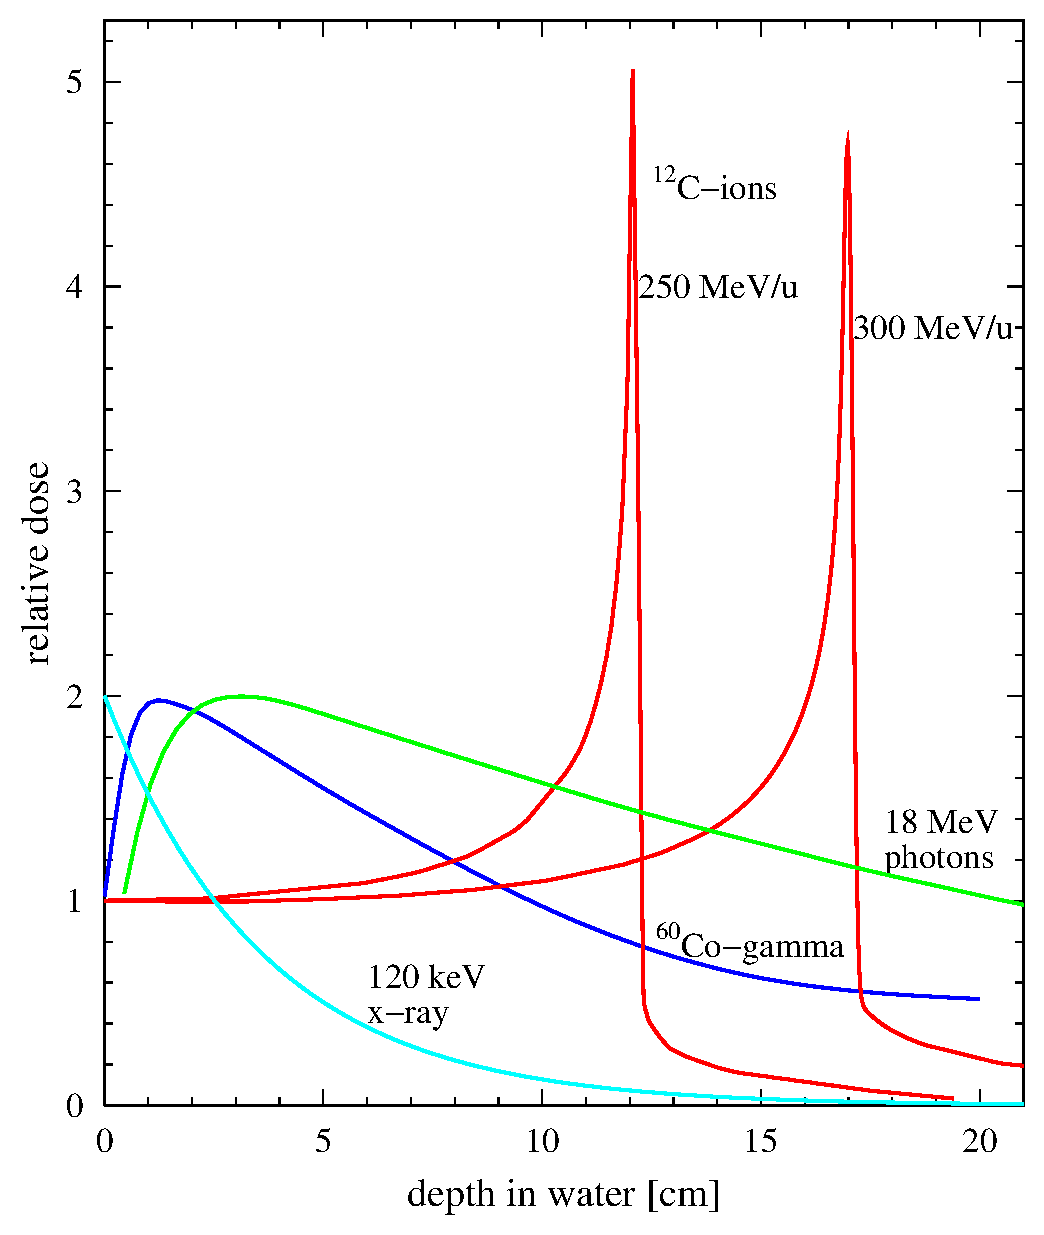
\includegraphics[scale=1]{depthdose.eps}
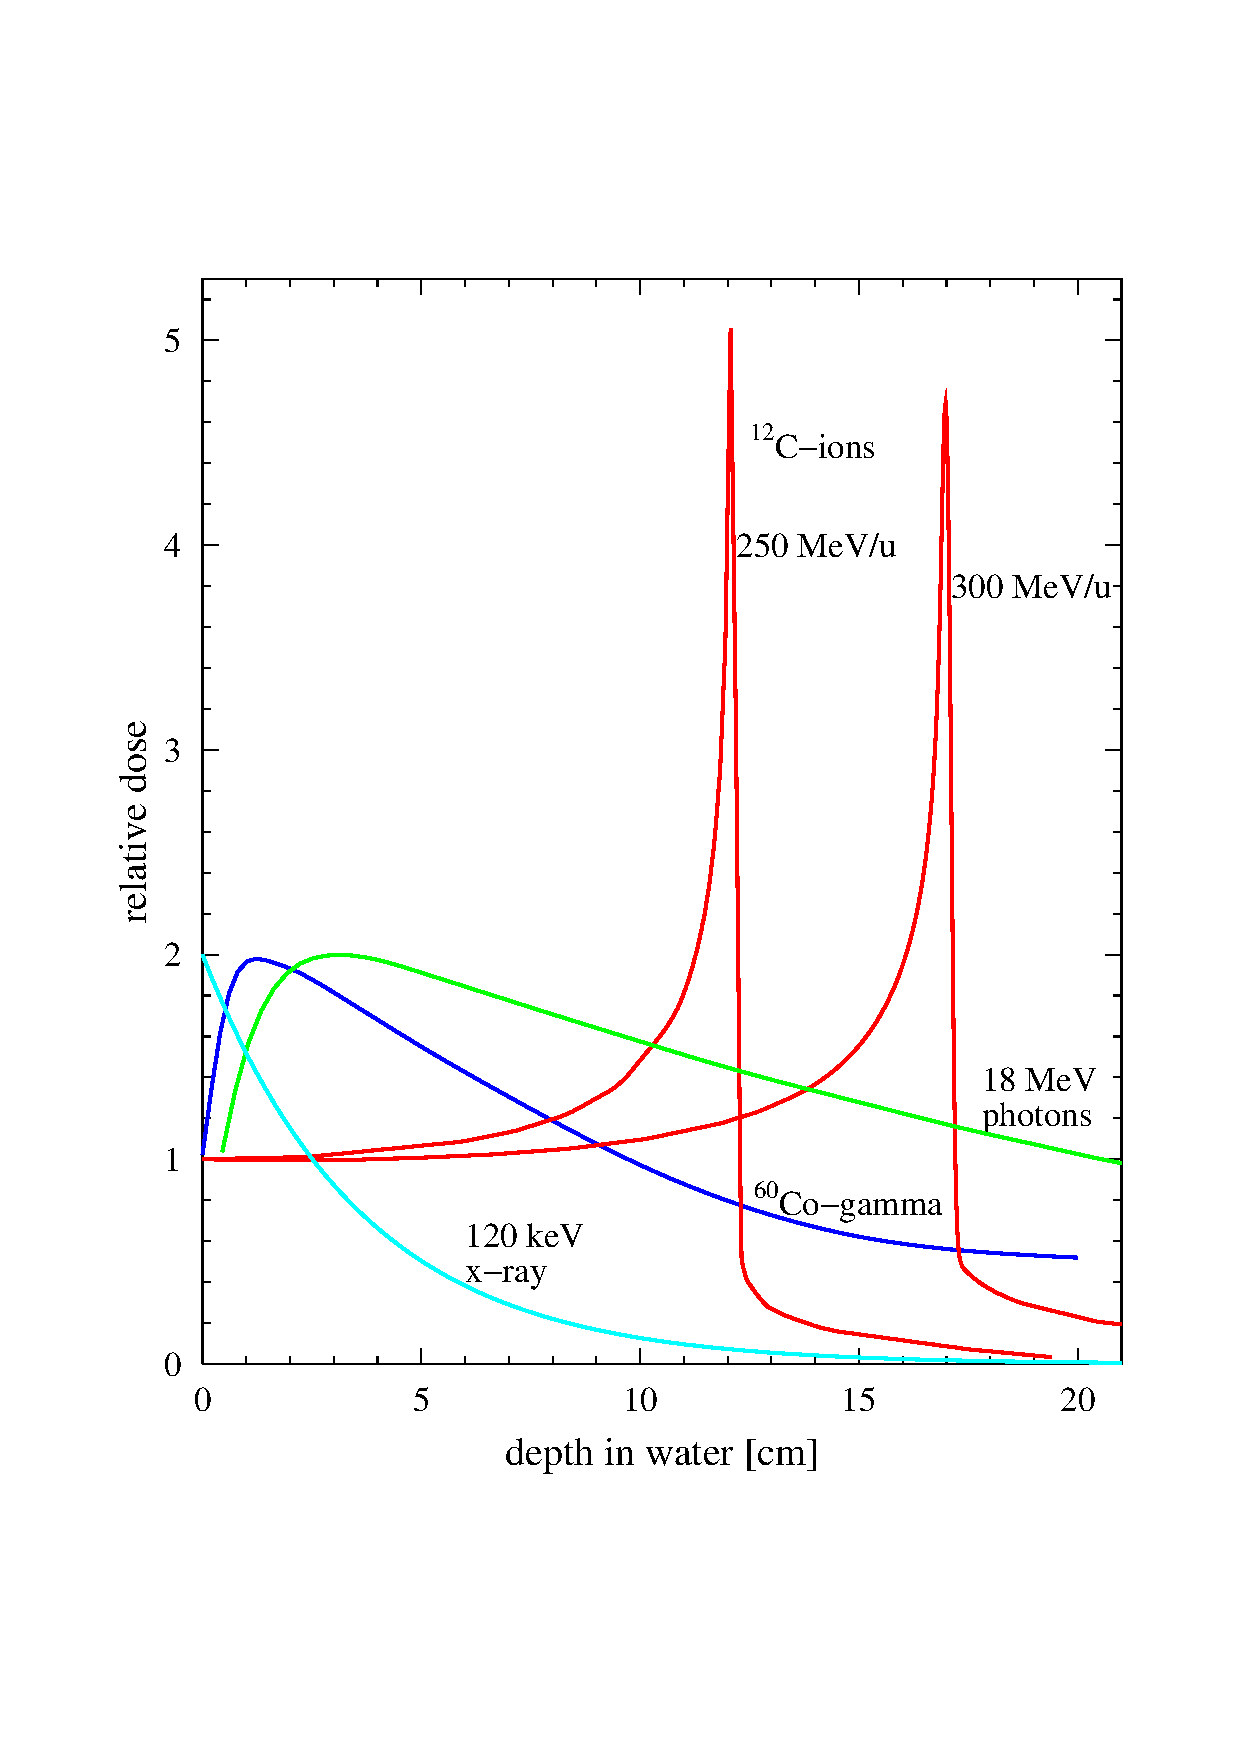
\includegraphics[scale=1]{./Images/depthdose.png}
\caption{Photon and carbon ions depth dose distributions at different energies. Photons start with a build up, which is followed by an exponential decrease after.
Ions deposit most of the dose at the end of the particle track, the Bragg peak. Figure taken from \cite{Schardt2010} }
\label{ddp}
\end{center}
\end{figure}


\subsubsection{Interaction of photons with matter}

Photons mostly interact with matter in one of the following ways: coherent or Rayleigh scattering, photoelectric effect, Compton scattering and pair production. The cross section, $\sigma$, for each of these processes depends
as well on the energy of the indicent photons as on the atomic number of the absorbin material \cite{Lilley2006}. The decreasing photon intesity in matter, $I$, can be described as:


\begin{equation}
 I = I_{0} \cdot e^{- N \sigma x} = I_{0} \cdot e^{-\mu x}
 \label{expdecrease}
\end{equation} 

where $I_{0}$ stands for the initial intensity of the photons, $x$ the depth of the material in units of length, $N$ the atomic density of the material and $\mu$ is the attenuation coefficient. The cross section, $sigma$ is the sum of all
possibile Interaction processes.

\begin{equation}
{\sigma} = \sigma_{rayleigh} + \sigma_{photoelectric} + Z\sigma_{compton} + \sigma_{pairproduction} 
\end{equation}

The energy range of photons used in radiotherapy is between 100 keV and 25 MeV. The dominating process in this energy range is Compton scattering \cite{Alpen1998}.
The electrons resulting from Compton interaction scatter mostly in a forward direction. Therefore a maximum of the depth-dose profile occurs when electons stop at a certain depth, 
the mean electron range. After this build up the dose deposition decreases exponentially (see figure \ref{ddp} and eq. \ref{expdecrease}).


\subsubsection{Interaction of ions with matter}
\label{iion}
Ions can interact with matter either with elastic columb scattering from target nuclei (nuclear stopping) or with inelastic collision with target electorns (electronic stopping).
At the ion energies used in radiotherapy, which are less then 500$\mathrm{MeV}/\mathrm{u}$, the electronic stoping is the dominated interaction. This results in ionization and excitation of the atoms in target.

The mean rate of ions energy loss in matter is described by the Bethe-Bloch formula \cite{Bethe1930, Bloch1933}. Since we are interested in low ion energies, we can make the following approximation:

\begin{equation}
- \left \langle \frac{dE}{dx} \right \rangle = \frac{ 4 \pi N_{e} z_{eff}^{2} }{ m_{e} v^{2} } \left( \frac{e^{2}}{4\pi \epsilon_{0}} \right) ^{2} \left[ln \left( \frac{2m_{e}v^{2}}{I} \right)+correction \right]
 \label{bethe}
\end{equation}

here $N_{e}$ is the materials electron density, $e$ and $m_{e}$ are the charge and mass 
of an electron, $\epsilon_{0}$ the electrical field constant and $I$ the mean excitation energy of the absorber material. 
Barkas formula \cite{Barkas1963} can be used for the approximation of the effective projectile charge $z_{eff}$: 

% \vspace*{-0.8cm}
\begin{equation}
 z_{eff} = z \left( 1 - e^{-125 \beta z^{\frac{2}{3}}} \right)
\end{equation}

where $\beta$ is the projectile speed in units of $c$.

The energy loss of ions is proportional to $z_{eff}$ and inversely proportional to $v^2$. The shape of the curve in figure \ref{ddp} can now be understood. Ions enter the matter with a high velocity,
resulting in a small energy deposition. Their velocity gradualy decreases, which in turn increases the energy deposition. The maximum of the energy loss is called Bragg peak or particle range.

\subsubsection{Lateral scattering and range straggling of ions}
\label{scat}
As mentioned in section \ref{iion} ions interact mostly via electronic stopping at energies used in radiotherapy. However, nuclear stopping still occurs and it is the main reason for lateral scattering.
The angular spread of ions is dependent on the mass of the target nuclei and on the momentum of the indecient ions \cite{Moliere1948}. The lateral scattering is proportional to mass of the target nuclei and inversely proportional
on the momentum of indecient ions. Carbon ions have thus less lateral scatter then protons. Experiments have shown that carbon ions have three times smaller angular spread compared to protons at the same range in water 
(15.6 cm, 150 MeV/u protons and 285 MeV/u $^{12}$C ions) \cite{Schardt2010}.

Statistical fluctuations of specific electronic stopping events cause range straggling of ions. If the number of collisions is high or the material is thick enoguh these fluctuations can be approximated by
a Gaussian probability distribution \cite{Bohr1940, Ahlen1980}. The straggling width $\sigma_R$ is proportional to:

\begin{equation}
 \sigma_R \propto R/\sqrt{M}
\end{equation}

where $R$ is the mean range of ions and $M$ the ion mass. Thus, the heavier the ion is, the less range straggling it has. Carbon ions have 3.5 smaller range straggling when compared to protons \cite{Schardt2010}.

\subsubsection{Nuclear fragmentation}
\label{nuclfrag}

Projectile ions (except protons) can be fragmented into ions with lower Z when transversing through matter. This becomes more important as projectile ions loose their energy, close to Bragg peak (see figure \ref{iondd}).
Fragments move in the same direction as projectile ions, with simmilar velocity. 
At large penetration depths, when the projectile ions have lost most of their energy, projectile fragmentation processes start to be 
relevant for ions heavier than protons. Mostly lower Z fragments are produced, which move with approximately the same velocity 
and in the same direction as the primary ions. This causes dose tails behind the Bragg peak position. Thus the resulting depth-dose 
distribution is actually the sum of the energy deposition of the projectiles and the resulting 
fragments. 

\begin{figure}[H]
\begin{center}
\includegraphics[scale=0.3]{./Images/iondepthdosesum.png}
\caption{Depth dose distribution of carbon ions. Besides of the energy deposition of the primary ions (red), the produced fragments 
(blue curve) contribute to the overall dose deposition (black) and are especially visible in the dose tail behind the Bragg 
peak. Figure taken from \cite{Groezinger2004}}
\label{iondd}
\end{center}
\end{figure}

Nevertheless, the produced fragments  also offer the chance for PET (Positron Emission Tomography) monitoring, 
without additional radiation exposure for the patient. As peripheral collisions are more frequent then central ones \cite{Kra00} 
isotopes like $^{11}C$ and $^{10}C$ are often produced when $^{12}C$ ions penetrate through tissue. Both isotopes are $\beta^{+}$ 
emitters. They annihilate with electrons in the human body, producing two $\gamma$-rays which travel in opposite directions.

% 
% \include{../ref.bib}
\bibliographystyle{apalike}
\bibliography{../ref.bib}{}
% \bibliographystyle{plain}

\end{document}